\chapter{Differential Equations}
    \subsection{Differential Equations}
        \begin{definition}
            A differential equation is an equation involving an unknown
            function and its derivatives.
        \end{definition}
        \begin{definition}
            An ordinary differential equation is a differential
            equation involving only ordinary derivatives.
        \end{definition}
        \begin{definition}
            A partial differential equation is an equation involving
            a function and its partial derivatives.
        \end{definition}
        \begin{definition}
            The order of a differential equation is the order
            of the highest derivative in the equation.
        \end{definition}
        \begin{definition}
            The degree of a differential equation is the highest exponent
            of the unknown function that appears in the equation.
        \end{definition}
        \begin{definition}
            A linear $n^{th}$ differential equation is an equation of the
            form $\sum_{k=0}^{n}a_{k}(x)y^{(n)}(x)=b(x)$, where
            $a_{n}(x)$ is not the zero function.
        \end{definition}
        First order linear differential equations have a
        simple method for solution:
        \begin{subequations}
            \begin{align}
                \dot{y}(x)+P(x)y(x)&=Q(x)\\
                \Rightarrow
                \exp\Big(\int^{x}P(\tau)\diff{\tau}\Big)
                \Big(\dot{y}(x)+P(x)y(x)\Big)
                &=\exp\Big(\int^{x}P(\tau)\diff{\tau}\Big)Q(x)\\
                \Rightarrow
                \frac{\diff}{\diff{x}}\bigg(
                    \exp\Big(\int^{x}P(\tau)\diff{\tau}\Big)
                    y(x)\bigg)
                &=\exp\Big(\int^{x}P(\tau)\diff{\tau}\Big)Q(x)
            \end{align}
        \end{subequations}
        Integrating across this, we get:
        \begin{equation}
            \exp\Big(\int^{x}P(\tau)\diff{\tau}\Big)y(x)
            =\int^{x}\exp\Big(\int^{\tau}P(\xi)\diff{\xi}\Big)
                Q(\tau)\diff{\tau}
        \end{equation}
        From this we obtain:
        \begin{equation}
            y(x)=\exp\Big(\minus\int^{x}P(\tau)\diff{\tau}\Big)
                \int^{x}\exp\Big(\int^{\tau}P(\xi)\diff{\xi}\Big)
                Q(\tau)\diff{\tau}
        \end{equation}
        The integration over $\tau$ and $\xi$ are just dummy variables.
        If we define $\mu$ to be:
        \begin{equation}
            \mu(x)=\exp\Big(\int^{x}P(\tau)\diff{\tau}\Big)    
        \end{equation}
        We can write this as:
        \begin{equation}
            y(x)=\frac{1}{\mu(x)}\int\mu(x)Q(x)\diff{x}+C
        \end{equation}
        \begin{lexample}
            The case with constant coefficients is easy to study:
            \begin{subequations}
                \begin{align}
                    \dot{y}(x)+ay(x)&=0\\
                    \Rightarrow{y(x)}&=C\exp(\minus{a}x)
                \end{align}
            \end{subequations}
            If we introduce a \textit{forcing function}, we obtain:
            \begin{subequations}
                \begin{align}
                    \dot{y}(x)+ay(x)&=g(x)\\
                    \label{eqn:Diff_EQ_Sol_to_FOLDE_Const_Coeff_Forced}
                    \Rightarrow{y(x)}
                    &=\exp(\minus{a}x)\int\exp(ax)g(x)\diff{x}
                    +C\exp(\minus{a}x)
                \end{align}
            \end{subequations}
            For a general function $g$ it may be
            difficult to evaluate
            Eqn.~\ref{eqn:Diff_EQ_Sol_to_FOLDE_Const_Coeff_Forced},
            but in practice we can apply numerical methods to obtain
            approximate solutions.
        \end{lexample}
        A separable equation is one of the form:
        \begin{align*}
            M(x,y)+N(x,y)\frac{\diff{y}}{\diff{x}}&=0\\
            \Rightarrow{M(x)M(y)\diff{x}}
            +N(x)N(y)\diff{y}&=0
        \end{align*}
        We can then rewrite this as:
        \begin{equation*}
            \frac{M(x)}{N(x)}\diff{x}+\frac{N(y)}{M(y)}\diff{y}=0
        \end{equation*}
        The general solution is then:
        \begin{equation*}
            \int^{x}\frac{M(x)}{N(x)}\diff{x}+
            \int^{x}\frac{N(y)}{M(y)}\diff{y}=C
        \end{equation*}
        \begin{example}
            Let's solve $xy^{2}\diff{x}-(x+5)\diff{y}=0$.
            This is separable, and we can write:
            \begin{equation*}
                \frac{x}{x+5}\diff{x}-\frac{1}{y^{2}}\diff{y}=0
            \end{equation*}
            Integrating, we obtain the general solution:
            \begin{align*}
                \int\frac{x}{x+5}\diff{x}-\int\frac{1}{y^{2}}
                &=C\\
                \Rightarrow
                x-5\ln|x+5|+\frac{1}{y}&=C\\
                \Rightarrow
                y&=\frac{1}{C-x+5\ln|x+5|}
            \end{align*}
        \end{example}
        \begin{definition}
            An exact equation is an equation of the form
            $M(x,y)\diff{x}+N(x,y)\diff{y}=0$ such that
            $\partial{M}/\partial{y}=\partial{N}/\partial{x}$.
        \end{definition}
        \begin{theorem}
            If $M(x,y)\diff{x}+N(x,y)\diff{y}=0$ is exact,
            then there exists an $F(x,y)$ such that:
            \begin{align*}
                \frac{\partial{F}}{\partial{x}}(x,y)&=M(x,y)
                &
                \frac{\partial{F}}{\partial{y}}(x,y)&=N(x,y)
            \end{align*}
        \end{theorem}
        We can integrate $F$ obtaining:
        \begin{equation*}
            F(x,y)=\int{M(x,y)\diff{x}}+g(y)
        \end{equation*}
        Where $g$ is a function of integration, obtained
        since we are taking partial derivatives.
        If $M(x,y)\diff{x}+N(x,y)\diff{y}$ is not exact, we
        often seek for a multiplication factor $\mu(x,y)$ such that
        $\mu(x,y)M(x,y)\diff{x}+\mu(x,y)N(x,y)\diff{y}$ is exact.
        \begin{theorem}
            If $M_{y}/N=N_{x}/N$ and $M_{y}/N$ is a function of
            $x$ alone, then $\mu(x)=\exp(\int{M_{y}/N}\diff{x}$ is
            the integrating factor.
        \end{theorem}
        \begin{theorem}
            If $M_{y}/M=N_{x}/M$, and
            $M_{y}/M$ is a function of $y$ alone, then
            $\mu(x)=\exp(-\int{M_{y}/M}\diff{y}$ is the
            integrating factor.
        \end{theorem}
        \begin{theorem}
            If $M_{x}+N_{y}\ne{0}$, then
            $\mu(x,y)=(M_{x}+N_{y})^{-1}$ is
            the integrating factor.
        \end{theorem}
        \begin{theorem}
            If $M(x,y)=yf(x,y)$, and
            $N(x,y)=xg(x,y)$, and if
            $f(x,y)\ne{g(x,y)}$, then the
            integrating factor is
            $\mu(x,y)=(M_{x}+N_{y})^{-1}$.
        \end{theorem}
        \begin{example}
            We can convert many types of equations into exact
            equations:
            \begin{equation*}
                x\diff{y}-y\diff{x}=0
                \Rightarrow\frac{x\diff{y}-y\diff{x}}{x^{2}}=0
                \Rightarrow\diff\big(\frac{y}{x}\big)=0
                \Rightarrow{y=Cx}
            \end{equation*}
            \begin{equation*}
                x\diff{y}-y\diff{x}=0
                \Rightarrow\frac{x\diff{y}-y\diff{x}}{xy}=0
                \Rightarrow\frac{\diff{y}}{y}-\frac{\diff{x}}{x}=0
                \Rightarrow\diff\ln\big(\frac{y}{x}\big)=0
                \Rightarrow{y=Cx}
            \end{equation*}
        \end{example}
        A homogeneous equation is an equation $y'(x)=f(x,y)$
        that depends only on the ratio $y/x$ or $x/y$.
        Letting $y=vx$, we have $y'(x)=xv'(x)+v(x)$.
        Substituting this back into our equation, we have:
        $xv'(x)+v(x)=F(v)$. This is separable and can be solved
        by direct integration. After solving, substitute
        $v=y/x$ again, and obtain the solution. A function $f(x,y)$
        is called homogeneous of degree $n$ if
        $f(\lambda{x},\lambda{y})=\lambda^{n}f(x,y)$.
        \begin{example}
            Solve $xy-y^{2}-x^{2}y'=0$. Dividing by $x^{2}$,
            we have:
            \begin{equation*}
                \frac{\diff{y}}{\diff{x}}(x)
                =\frac{y}{x}-\frac{y^{2}}{x^{2}}
            \end{equation*}
            Let $y=vx$. Then $y'(x)=xv'(x)+v$, so we have:
            \begin{equation*}
                x\frac{\diff{v}}{\diff{x}}+v=v-v^{2}
            \end{equation*}
            Simiplifying, we have:
            \begin{equation*}
                \frac{\diff{v}}{\diff{x}}+\frac{v^{2}}{x}=0
            \end{equation*}
            Solving, we get $v=(C-\ln|x|)^{-1}$.
            But $v=y/x$, so we have:
            \begin{equation*}
                y=\frac{x}{C-\ln(x)}
            \end{equation*}
        \end{example}
        A second order differential equation is one involving
        the second derivatives of the unknown function. A simple
        boundary value problem on the interval $(a,b)$ is
        $y''(x)+P(x)y'(x)+Q(x)y(x)=F(x)$, where
        $y(a)=y_{0}$ and $y(b)=y_{1}$. The homogeneous solution
        is $y''(x)+P(x)y'(x)+Q(x)y(x)=0$. From the linearity of
        the problem, if $y_{h}(x)$ is the homogeneous solution,
        and $y_{p}$ solves the original problem, then
        $C_{1}y_{p}+C_{2}y_{h}$ is a solution as well, for
        arbitrary constants $C_{1}$ and $C_{2}$. The Wronskian
        of these two solutions is $y_{h}y_{p}'-y_{h}'y_{p}$.
        The Wronskian is either the zero function, or is
        never zero. Reduction of order allows a second order
        differential equation to be converted into a first
        order differential equation, if a solution is already
        known. If $y''(x)+P(x)y'(x)+Q(x)y(x)=0$, and if
        $y_{1}(x)$ is a known solution, a second
        solution of the form $y_{2}=u(x)y_{1}(x)$ can be
        determined. Substituting this in, we have
        $u''(x)+(P(x)+2y'(x)/y(x))u'(x)=0$. This is a first
        order differential equation in terms of the variable
        $u'(x)$. The solution is
        $u'(x)=C\exp(-\int(p(x)+y'(x)/y(x))\diff{x})$.
        Integrating this gives the second solution.
        The general solution is then
        $y=C_{1}y_{1}(x)+C_{2}y_{2}(x)$. Another common
        second order differential equation is one with
        constant coefficients. If 
        $ay''+by'+cy=0$, we look at the characteristic
        polynomail of the equation:
        $ar^{2}+br+c=0$, and solve for the roots. We
        can do this using the quadratic formula. If
        the roots are real and distinct (That is,
        if $b^{2}-4ac>0$), then the general solution
        is $y=C_{1}\exp(r_{1}x)+C_{2}\exp(r_{2}x)$,
        where $r_{1}$ and $r_{2}$ are the roots. If
        both roots are identical (That is,
        if $b^{2}-4ac=0$), then the general solution
        is $y(x)=C_{1}\exp(rx)+C_{2}x\exp(rx)$. Finally,
        if the roots are complex (That is, if
        $b^{2}-4ac<0$), then the general solution is of
        the form
        $y(x)=\exp(\lambda{x})(C_{1}\sin(\mu{x})+C_{2}\cos(\mu{x})$,
        where $\lambda=b/2a$, and $\mu=\sqrt{b^{2}-4ac}/2a$.
        The last method to be discussed is that of
        variation of parameters. This is also called
        Lagrange's Method. If $y''(x)+P(x)y'(x)+Q(x)y(x)=f(x)$,
        and if $y_{1}$ and $y_{2}$ are solutions
        to the homogeneous equation $f(x)=0$, then the particular
        solution is of the form $y=u_{1}y_{1}+u_{2}y_{2}$ such
        that $u_{1}'(x)y_{1}(x)+u_{2}'(x)y_{2}(x)=0$
        and $u_{1}'(x)y_{1}'(x)+u_{2}'(x)y_{2}'(x)=f(x)$.
        The general solution is thus:
        \begin{equation*}
            y_{p}=
            -y_{1}(x)\int\frac{y_{2}(x)f(x)}{W(y_{1},y_{2})}\diff{x}
            +y_{2}(x)\int\frac{y_{1}(x)f(x)}{W(y_{1},y_{2})}\diff{x}
        \end{equation*}
    \section{Systems of Differential Equations}
        \subsection{Linear First Order Systems}
            Ordinary differential equations involve equations
            relating a function to its derivatives. These
            usually involve real-valued functions that
            we we can think of as graphs in the $xy$ plane. 
            Systems of differential equations arise when we
            consider several differential equations in several
            different functions. For example:
            \par\hfill\par
            \vspace{-1ex}
            \begin{subequations}
                \begin{minipage}{0.49\textwidth}
                    \begin{equation}
                        \dot{x}(t)
                        =f_{1}(t,x(t),y(t))
                    \end{equation}
                \end{minipage}
                \hfill
                \begin{minipage}{0.49\textwidth}
                    \begin{equation}
                        \dot{y}(t)
                        =f_{2}(t,x(t),y(t))
                    \end{equation}
                \end{minipage}
            \end{subequations}
            \par\hfill\par
            Where $\dot{x}(t)$ denotes the derivative of $x$
            with respect to $t$, and similarly for $\dot{y}$.
            The most basic case to study is when both
            $f_{1}$ and $f_{2}$ are linear functions of
            $x(t)$ and $y(t)$ with constant coefficients.
            We obtain:
            \par\hfill\par
            \vspace{-1ex}
            \begin{subequations}
                \begin{minipage}{0.49\textwidth}
                    \begin{equation}
                        \label{diffeq:Simply_Linear_Coupled_Eq_1}
                        \dot{x}(t)
                        =ax(t)+by(t)
                    \end{equation}
                \end{minipage}
                \hfill
                \begin{minipage}{0.49\textwidth}
                    \begin{equation}
                        \label{diffeq:Simply_Linear_Coupled_Eq_2}
                        \dot{y}(t)
                        =cx(t)+dy(t)
                    \end{equation}
                \end{minipage}
            \end{subequations}
            \par\hfill\par
            We can rewrite this system as a single
            vector-valued differential equation.
            Let $Y$ and $A$ be defined as:
            \par\hfill\par
            \vspace{-1ex}
            \begin{subequations}
                \begin{minipage}{0.49\textwidth}
                    \begin{equation}
                        \label{diffeq:Vector_Rep_for_Coupled_Eq}
                        Y(T)=
                        \begin{bmatrix}
                            x(t)\\
                            y(t)
                        \end{bmatrix}
                    \end{equation}
                \end{minipage}
                \hfill
                \begin{minipage}{0.49\textwidth}
                    \begin{equation}
                        \label{diffeq:Coupled_Coefficient_Matrix}
                        A=
                        \begin{bmatrix}
                            a&b\\
                            c&d
                        \end{bmatrix}
                    \end{equation}
                \end{minipage}
            \end{subequations}
            \par\hfill\par
            Using this, we can rewrite our system of
            differential equations as:
            \begin{equation}
                \dot{Y}(t)=AY(t)
            \end{equation}
            Using the exponential of the matrix $A$
            we can solve this vector-valued differential
            equation and obtain a general solution.
            We can also solve this without the use of linear
            algebra, and we'll take that approach for now. Using
            Eqn.~\ref{diffeq:Simply_Linear_Coupled_Eq_1}
            we see that if $x(t)$ is a solution to this system
            of a differential equations then it must be twice
            differentiable. That is, $\ddot{x}(t)$ is well defined.
            For $\dot{x}(t)=ax(t)+by(t)$, and $x(t)$ and
            $y(t)$ are differentiable, and therefore $\dot{x}(t)$
            is differentiable. We can use this to obtain a
            second-order linear differential equation in $x(t)$
            alone. We have:
            \begin{equation}
                \ddot{x}(t)=a\dot{x}(t)+b\dot{y}(t)
            \end{equation}
            But from Eqn.~\ref{diffeq:Simply_Linear_Coupled_Eq_2},
            $\dot{y}(t)=cx(t)+dy(t)$. By rearranging
            Eqn.~\ref{diffeq:Simply_Linear_Coupled_Eq_1} we have
            $by(t)=\dot{x}(t)-ax(t)$, and therefore
            $bdy(t)=d\dot{x}(t)-adx(t)$. From this we obtain:
            \begin{subequations}
                \begin{align}
                    \ddot{x}(t)
                    &=a\dot{x}(t)+b\big(cx(t)+dy(t)\big)\\
                    \Rightarrow\ddot{x}(t)
                    &=(a+d)\dot{x}(t)-(ad-bc)x(t)
                \end{align}
            \end{subequations}
            Recall from linear algebra that the trace of a
            matrix is the sum of the diagonal components. Using
            the matrix $A$ we defined before
            (Eqn.~\ref{diffeq:Coupled_Coefficient_Matrix})
            we can rewrite this second-order linear differential
            equation in terms of the determinant
            $\det(A)$ and the trace $\Tr(A)$ of $A$.
            \begin{equation}
                \label{diffeq:Coupled_Simple_Second_Ord_DE}
                \ddot{x}(t)-\Tr(A)\dot{x}(t)+\det(A)x(t)=0
            \end{equation}
            We now must prove that
            Eqn.~\ref{diffeq:Coupled_Simple_Second_Ord_DE} has
            a solution and, given initial conditions, that the
            solution is unique.
            \begin{ftheorem}{}{diffeq:Sol_Second_Order_Lin_DE_Pos}
                If $x(t)$ is a twice differentiable function,
                $x_{0}=x(0)$, $\dot{x}_{0}=\dot{x}(0)$, and if
                there are constants $a,b\in\mathbb{R}$ such that
                $a^{2}-4b>0$ and
                $\ddot{x}(t)+a\dot{x}(t)+bx(t)=0$ for all
                $t\in\mathbb{R}$, then:
                \begin{equation*}
                    x(t)=
                    C_{1}\exp\Big(\frac{-a+\sqrt{a^{2}-4b}}{2}t\Big)
                    +
                    C_{2}\exp\Big(\frac{-a-\sqrt{a^{2}-4b}}{2}t\Big)
                \end{equation*}
                Where:
                \begin{align*}
                    C_{1}&=
                    \frac{1}{2\sqrt{a^{2}-4b}}\Big(
                    \big(a+\sqrt{a^{2}-4b}\big)x_{0}+
                    2\dot{x}_{0}\Big)\\
                    C_{2}&=
                    \frac{1}{2\sqrt{a^{2}-4b}}\Big(
                    \big(-a+\sqrt{a^{2}-4b}\big)x_{0}-
                    2\dot{x}_{0}\Big)
                \end{align*}
            \end{ftheorem}
            \begin{bproof}
                We will use one of the fundamental results from
                the theory of differential equations to prove this.
                If the \textit{Wronskian} of two functions $x_{1}$
                and $x_{2}$ is non-zero, then the general solution
                to the differential equation is
                $C_{1}x_{1}(t)+C_{2}x_{2}(t)$. Define $x_{1}(t)$
                and $x_{2}(t)$ as follows:
                \begin{align*}
                    x_{1}(t)&=
                    \exp\Big(\frac{-a+\sqrt{a^{2}-4b}}{2}t\Big)
                    &
                    x_{2}(t)&=
                    \exp\Big(\frac{-a-\sqrt{a^{2}-4b}}{2}t\Big)
                \end{align*}
                The Wronskian $W(x_{1},x_{2})$ is defined as:
                \begin{equation*}
                    W(x_{1},x_{2})=\det\bigg(
                    \begin{bmatrix}
                        x_{1}(t)&x_{2}(t)\\
                        \dot{x}_{1}(t)&\dot{x}_{2}(t)
                    \end{bmatrix}
                    \bigg)
                    =x_{1}(t)\dot{x}_{2}(t)-\dot{x}_{1}(t)x_{2}(t)
                \end{equation*}
                From the definition of $x_{1}$ and $x_{2}$,
                the Wronskian is non-zero. Moreover, both $x_{1}$
                and $x_{2}$ satisfy the differential equation.
                For let $r_{1}=\frac{-a+\sqrt{a^{2}-4b}}{2}$
                and let $r_{2}=\frac{-a-\sqrt{a^{2}-4b}}{2}$.
                Then:
                \begin{equation*}
                    \ddot{x}_{1}(t)+a\dot{x}_{1}(t)+bx_{1}(t)
                    =\exp(r_{1}t)\big(r_{1}^{2}+ar_{1}+b\big)
                \end{equation*}
                But $r_{1}$ is a root of the polynomial
                $r^{2}+ar+b$, and thus
                $\ddot{x}_{1}(t)+a\dot{x}_{1}(t)+bx_{1}(t)=0$.
                Similarly, $x_{2}(t)$ satisfies the differential
                equation since $r_{2}$ is also a root of this
                polynomial. And since the Wronskian
                of $x_{1}$ and $x_{2}$ is non-zero, any solution
                is of the form:
                \begin{equation*}
                    x(t)=C_{1}x_{1}(t)+C_{2}x_{2}(t)
                \end{equation*}
                Solving for the coefficients, we use the initial
                values given and obtain the following system of
                equations:
                \begin{align*}
                    \phantom{\Big(\frac{-a+\sqrt{a^{2}-4b}}{2}\Big)}
                    C_{1}+
                    \phantom{\Big(\frac{-a+\sqrt{a^{2}-4b}}{2}\Big)}
                    C_{2}&=x_{0}\\
                    \Big(\frac{-a+\sqrt{a^{2}-4b}}{2}\Big)C_{1}+
                    \Big(\frac{-a-\sqrt{a^{2}-4b}}{2}\Big)C_{2}
                    &=\dot{x}_{0}
                \end{align*}
                The coefficient matrix is invertible
                since $a^{2}-4b>0$. Solving, we obtain:
                \begin{align*}
                    C_{1}&=
                    \frac{1}{2\sqrt{a^{2}-4b}}\Big(
                    \big(a+\sqrt{a^{2}-4b}\big)x_{0}+
                    2\dot{x}_{0}\Big)\\
                    C_{2}&=
                    \frac{1}{2\sqrt{a^{2}-4b}}\Big(
                    \big(-a+\sqrt{a^{2}-4b}\big)x_{0}-
                    2\dot{x}_{0}\Big)
                \end{align*}
            \end{bproof}
            We have thus solved the case for when $a^{2}-4b>0$.
            There are two cases left, when $a^{2}-4b=0$ and when
            $a^{2}-4b<0$. In the case of equality, we call the
            differential equation \textit{degenerate}. The reason
            being is that the two independent solutions we found
            before will now be the same function. That is,
            we'll obtain $x_{1}(t)=\exp(-at/2)$ and
            $x_{2}(t)=\exp(-at/2)$. The Wronskian will thus be
            zero, and we won't be able to use this to obtain
            the general solution. For the case of degeneracy
            we will have to be a little more clever. When we have
            $a^{2}-4b<0$ we can apply the same method, but we
            will have to use different functions if we want to
            avoid using imaginary numbers. If we don't care about
            using $i=\sqrt{-1}$, then we can use the previous
            solution and invoke Euler's Formula.
            \begin{ftheorem}{Euler's Formula}{diffeq:Euler_Formula}
                If $\theta$ is a real number, then:
                \begin{equation*}
                    \exp(i\theta)=\cos(\theta)+i\sin(\theta)
                \end{equation*}
            \end{ftheorem}
            \begin{bproof}
                Using the Taylor expansion for $\exp(i\theta)$
                about the origin, we have:
                \begin{equation*}
                    \exp(i\theta)
                    =\sum_{n=0}^{\infty}\frac{(i\theta)^{n}}{n!}
                \end{equation*}
                There are four cases to consider for $i^{n}$:
                \begin{equation*}
                    i^{n}=
                    \begin{cases}
                        i,&n\mod{4}=1\\
                        -1,&n\mod{4}=2\\
                        -i,&n\mod{4}=3\\
                        1,&n\mod{4}=0
                    \end{cases}
                \end{equation*}
                We can therefore split the sum into two parts:
                \begin{align*}
                    \exp(i\theta)
                    &=\sum_{n=0}^{\infty}\frac{(i\theta)^{n}}{n!}\\
                    &=\sum_{n=0}^{\infty}
                    \frac{(-1)^{n}\theta^{2n}}{(2n)!}+
                    i\sum_{n=0}^{\infty}
                    \frac{(-1)^{n}\theta^{2n+1}}{(2n+1)!}
                \end{align*}
                But the left sum is just the Taylor expansion
                for $\cos(\theta)$ about the origin, and the
                right sum is the Taylor expansion for
                $i\sin(\theta)$ about the origin. Combining these
                we get
                $\exp(i\theta)=\cos(\theta)+i\sin(\theta)$.
            \end{bproof}
            \begin{fcorollary}{}{}
                If $a$ and $b$ are real numbers, then:
                \begin{equation*}
                    \exp(a+ib)=\exp(a)\big(\cos(b)+i\sin(b)\big)
                \end{equation*}
            \end{fcorollary}
            \begin{bproof}
                For
                $\exp(a+ib)=\exp(a)\exp(ib)%
                 =\exp(a)(\cos(b)+i\sin(b))$
            \end{bproof}
            Using this we can solve the differential equation
            $\ddot{x}(t)+a\dot{x}(t)+bx(t)$ for whenever
            $a^{2}-4b\ne{0}$. If we want to avoid using
            complex numbers, Euler's formula also gives us a
            hint as to what we should choose for
            $x_{1}$ and $x_{2}$ in the case of
            $a^{2}-4b<0$. That is, a good guess would be
            $x_{1}=\exp(At)\cos(Bt)$ and
            $x_{2}=\exp(At)\sin(Bt)$. The problem is now which
            $A$ and $B$ will work?
            \begin{ftheorem}{}{diffeq:Sol_Second_Order_Lin_DE_Neg}
                If $x(t)$ is a twice differentiable function,
                $x_{0}=x(0)$, $\dot{x}_{0}=\dot{x}(0)$, and if
                there are constants $a,b\in\mathbb{R}$ such that
                $a^{2}-4b<0$ and
                $\ddot{x}(t)+a\dot{x}(t)+bx(t)=0$ for all
                $t\in\mathbb{R}$, then:
                \begin{equation*}
                    x(t)=\exp(-\frac{a}{2}t)\bigg(
                    C_{1}\cos\Big(\frac{\sqrt{4b-a^{2}}}{2}t\Big)+
                    C_{2}\sin\Big(\frac{\sqrt{4b-a^{2}}}{2}t\Big)
                    \bigg)
                \end{equation*}
                Where:
                \begin{align*}
                    C_{1}&=x_{0}
                    &
                    C_{2}
                    &=\frac{2\dot{x}_{0}
                    +ax_{0}}{\sqrt{4b-a^{2}}}
                \end{align*}
            \end{ftheorem}
            \begin{bproof}
                The proof is similar to the proof of
                Thm.~\ref{th:diffeq:Sol_Second_Order_Lin_DE_Pos}.
                Define the following:
                \par
                \vspace{-1ex}
                \begin{minipage}{0.49\textwidth}
                    \begin{equation*}
                        x_{1}(t)=\exp(-at/2)
                        \cos\Big(\frac{\sqrt{4b-a^{2}}}{2}t\Big)
                    \end{equation*}
                \end{minipage}
                \hfill
                \begin{minipage}{0.49\textwidth}
                    \begin{equation*}
                        x_{2}(t)=\exp(-at/2)
                        \sin\Big(\frac{\sqrt{4b-a^{2}}}{2}t\Big)
                    \end{equation*}
                \end{minipage}
                \par\hfill\par
                The Wronskian $W(x_{1},x_{2})$ is non-zero, and
                both $x_{1}$ and $x_{2}$ satisfy the
                differential equation. The general solution is then
                $x(t)=C_{1}x_{1}(t)+C_{2}x_{2}(t)$. Evaluating
                $x(t)$ and $\dot{x}(x)$ at $t=0$ gives us the
                values of $C_{1}$ and $C_{2}$.
            \end{bproof}
            The final case to consider is that of degeneracy,
            when $a^{2}-4b=0$.
            We have already found one solution, for
            $x_{1}(t)=\exp(-at/2)$ satisfies the differential
            equation. For:
            \begin{equation}
                \ddot{x}_{1}(t)+a\dot{x}_{1}(t)+bx_{1}(t)
                =-\frac{1}{4}\exp(-at/2)\big(a^{2}-4b\big)
            \end{equation}
            But $a^{2}-4b=0$, so
            $\ddot{x}_{1}(t)+a\dot{x}_{1}(t)+bx_{1}(t)=0$.
            We now need to find a function $x_{2}(t)$ that
            satisfies the differential equation such that
            the Wronskian $W(x_{1},x_{2})$ is non-zero. We can
            start wildly guessing, but there is a very
            methodical technique available called
            \textit{reduction of order} that will always give
            you a second independent solution if you've already
            found a first. Before we get there, let's try wildly
            guessing and start with $x_{2}(t)=tx_{1}(t)$.
            That is, $x_{2}(t)=t\exp(-at/2)$. Then we have:
            \begin{subequations}
                \begin{align}
                    x_{2}(t)
                    &=t\exp\big(-\frac{at}{2}\big)\\
                    \dot{x}_{2}(t)
                    &=\exp\big(-\frac{at}{2}\big)
                    \Big(1-\frac{a}{2}t\Big)\\
                    \ddot{x}_{2}(t)
                    &=\exp\big(-\frac{at}{2}\big)
                    \Big(\frac{a^{2}}{4}t-a\Big)
                \end{align}
            \end{subequations}
            Piecing this together, we have:
            \begin{subequations}
                \begin{align}
                    \ddot{x}_{2}(t)+a\dot{x}_{2}(t)+bx_{2}(t)
                    &=\exp\big(-\frac{at}{2}\big)
                    \Big(\frac{a^{2}}{4}t-a+a-\frac{a^{2}}{2}t+bt\Big)\\
                    &=t\exp\big(-\frac{at}{2}\big)
                    \Big(b-\frac{a^{2}}{4}\Big)
                \end{align}
            \end{subequations}
            But $a^{2}=4b$, and thus $b=a^{2}/4$. Therefore
            $x_{2}(t)$ also satisfies the differential equation.
            Moreover, $x_{1}(t)$ and $x_{2}(t)$ are independent of
            each other, as the Wronskian $W(x_{1},x_{2})$ is
            non-zero. We now have the general solution for
            the degenerate case.
            \begin{ftheorem}{}{diffeq:Sol_Second_Order_Lin_DE_Deg}
                If $x(t)$ is a twice differentiable function,
                $x_{0}=x(0)$, $\dot{x}_{0}=\dot{x}(0)$, and if
                there are constants $a,b\in\mathbb{R}$ such that
                $a^{2}-4b=0$ and
                $\ddot{x}(t)+a\dot{x}(t)+bx(t)=0$, then:
                \begin{equation*}
                    x(t)=\exp\big(-\frac{at}{2}\big)
                    \big(C_{1}+C_{2}t\big)
                \end{equation*}
                Where:
                \begin{align*}
                    C_{1}&=x_{0}
                    &
                    C_{2}&=\dot{x}_{0}+\frac{a}{2}x_{0}
                \end{align*}
            \end{ftheorem}
            \begin{bproof}
                For let $x_{1}(t)=\exp(-at/2)$ and
                $x_{2}(t)=t\exp(-at/2)$. Then $x_{1}(t)$ and
                $x_{2}(t)$ are both solutions to the
                differential equation and
                $W(x_{1},x_{2})$ is non-zero. Therefore the
                general solution is of the form
                $x(t)=C_{1}x_{1}(t)+C_{2}x_{2}(t)$. Evaluating
                $x(t)$ and $\dot{x}(t)$ at $t=0$ gives us
                $C_{1}$ and $C_{2}$.
            \end{bproof}
            With this, we have solved all three cases. If
            $a$ and $b$ are real numbers and if:
            \begin{equation*}
                \ddot{x}(t)+a\dot{x}(t)+bx(t)=0
            \end{equation*}
            Then:
            \begin{equation}
                \label{diffeq:gen_sol_to_sec_ord_lin_de_const_coeff}
                x(t)=
                \begin{cases}
                    C_{1}\exp
                    \big(\frac{-a-\sqrt{a^{2}-4b}}{2}t\big)+
                    C_{2}\exp\big(\frac{-a+\sqrt{a^{2}-4b}}{2}t\big)
                    &a^{2}-4b>0\\[2ex]
                    \exp\big(-\frac{at}{2}\big)
                    \big(C_{1}+C_{2}t\big)&a^{2}-4b=0\\[2ex]
                    \exp(-\frac{a}{2}t)\Big[
                    C_{1}\cos\big(\frac{\sqrt{4b-a^{2}}}{2}t\big)+
                    C_{2}\sin\big(\frac{\sqrt{4b-a^{2}}}{2}t\big)
                    \Big]&a^{2}-4b<0
                \end{cases}
            \end{equation}
            For second-order linear differential equations
            with non-constant coefficients, we need to modify
            our approach. Often it is easy to obtain
            one non-trivial solution to a given problem,
            and we are thus tasked with
            finding a second independent one. For the case of
            degeneracy we tried $x_{2}(t)=tx_{1}(t)$ and luckily
            that worked. In general guessing and checking is
            not the best method, and does not guarantee a
            solution. However, if we have a solution
            $x_{1}(t)$ to the differential equation, then we
            can obtain a second solution via reduction of order.
            We'll work backwards, trying to find a solution that
            works, and then after obtaining one that looks correct
            we'll show that it is rigorously. Suppose we have the
            following differential equation:
            \begin{equation}
                \label{diffeq:general_second_order_linear_DE}
                \ddot{x}(t)+p(t)\dot{x}(t)+q(t)x(t)=0
            \end{equation}
            Where $p(t)$ and $q(t)$ are continuous functions. Suppose we
            have found a non-trivial solution $x_{1}(t)$. By non-trivial,
            we mean that $x_{1}(t)$ is not identically equal to the
            zero function. To obtain the general solution to this
            differential equation we are tasked with finding a second
            function $x_{2}(t)$ that also satisfies
            Eqn.~\ref{diffeq:general_second_order_linear_DE}. Let's work
            backwards. Suppose there is a function $u(t)$ such that
            $x_{2}(t)=u(t)x_{1}(t)$ is a solution. What properties must
            $u(t)$ have? Differentiating, we have:
            \begin{subequations}
                \begin{align}
                    x_{2}(t)&=u(t)x_{1}(t)\\
                    \dot{x}_{2}(t)&=\dot{u}(t)x_{1}(t)+u(t)\dot{x}_{1}(t)\\
                    \ddot{x}_{2}(t)
                    &=\ddot{u}(t)x_{1}(t)+2\dot{u}(t)\dot{x}_{1}(t)
                    +u(t)\ddot{x}_{1}(t)
                \end{align}
            \end{subequations}
            Plugging this in to
            Eqn.~\ref{diffeq:general_second_order_linear_DE}, we have:
            \begin{align}
                \nonumber
                \ddot{x}_{2}(t)+p(t)\dot{x}_{2}(t)+q(t)x_{2}(t)
                =&\hspace{0.5em}\ddot{u}(t)x_{1}(t)+\\
                \nonumber&\hspace{0.5em}
                \dot{u}(t)\big(2\dot{x}_{1}(t)+p(t)x_{1}(t)\big)+\\
                &\hspace{0.5em}
                u(t)\big(\ddot{x}_{1}(t)+p(t)\dot{x}_{1}(t)+q(t)x_{1}(t)\big)
            \end{align}
            But $x_{1}(t)$ is a solution to
            Eqn.~\ref{diffeq:general_second_order_linear_DE}, and therefore
            $\ddot{x}_{1}(t)+p(t)\dot{x}_{1}(t)+q(t)x_{1}(t)=0$. But also
            we have imposed the requirement that $x_{2}(t)$ is also a
            solution. With this we obtain our reduced equation:
            \begin{equation}
                \label{diffeq:Reduc_of_Order_Reduced_Equation_in_u}
                x_{1}(t)\ddot{u}(t)+
                \big(2\dot{x}_{1}(t)+p(t)x_{1}(t)\big)\dot{u}(t)=0
            \end{equation}
            Let $v(t)$ be defined as follows:
            \begin{equation}
                \label{diffeq:reduction_term_v_of_u}
                v(t)=\dot{u}(t)
            \end{equation}
            Recall that $x_{1}(t)$ is not identically
            zero everywhere. So we can convert
            Eqn.~\ref{diffeq:Reduc_of_Order_Reduced_Equation_in_u}
            into the following first-order linear
            equations in $v(t)$:
            \begin{subequations}
                \begin{align}
                    x_{1}(t)\dot{v}(t)+
                    \big(2\dot{x}_{1}(t)+p(t)x_{1}(t)\big)v(t)&=0\\
                    \label{diffeq:reduction_of_order_first_order_ode}
                    \Rightarrow\dot{v}(t)+
                    \Big(2\frac{\dot{x}_{1}(t)}{x_{1}(t)}+p(t)\Big)v(t)
                    &=0
                \end{align}
            \end{subequations}
            Any first-order linear differential equation with
            continuous coefficients can be solved via the integrating
            factor. Actual evaluation of this integral may be very
            difficult in practice, but at the very least we obtain a means
            for numerical solutions. Let $\mu(t)$ be defined as:
            \begin{equation}
                \mu(t)=
                \exp\Big(\int_{t_{0}}^{t}
                    \big(2\frac{\dot{x}_{1}(\tau)}{x_{1}(\tau)}
                         +p(\tau)\big)\diff{\tau}\Big)
            \end{equation}
            We use $\tau$ to denote a dummy variable of integration. This is
            to avoid later confusion with the actual variable $t$.
            We can simplify $\mu(t)$ further as follows:
            \begin{subequations}
                \begin{align}
                    \exp\Big(2\int_{t_{0}}^{t}
                             \frac{\dot{x}_{1}(\tau)}{x_{1}(\tau)}
                             \diff{\tau}\Big)
                    &=\exp\Big(2\ln\big(\frac{x_{1}(t)}{x_{1}(t_{0})}\big)
                    \Big)\\
                    \Rightarrow\mu(t)
                    &=\Big(\frac{x_{1}(t)}{x_{1}(t_{0})}\Big)^{2}
                    \exp\Big(\int_{t_{0}}^{t}p(\tau)\diff{\tau}\Big)
                \end{align}
            \end{subequations}
            Using the product rule from Calculus, we see that:
            \begin{equation}
                \frac{\diff}{\diff{t}}\Big(v(t)\mu(t)\Big)
                =\mu(t)\Big(\dot{v}(t)+
                \big(2\frac{\dot{x}_{1}(t)}{x_{1}(t)}+p(t)\big)v(t)\Big)
            \end{equation}
            But from Eqn.~\ref{diffeq:reduction_of_order_first_order_ode},
            the right hand side of this equation is zero. Therefore:
            \par
            \begin{subequations}
                \begin{minipage}[b]{0.49\textwidth}
                    \centering
                    \begin{equation}
                        \frac{\diff}{\diff{t}}\Big(v(t)\mu(t)\Big)=0
                    \end{equation}
                \end{minipage}
                \hfill
                \begin{minipage}[b]{0.49\textwidth}
                    \centering
                    \begin{equation}
                        \Rightarrow
                        v(t)=\frac{C}{\mu(t)}
                    \end{equation}
                \end{minipage}
            \end{subequations}
            \par\hfill\par
            Where $C$ is some constant of integration. But from
            Eqn.~\ref{diffeq:reduction_term_v_of_u},
            $v(t)=\dot{u}(t)$. Using this, we obtain:
            \begin{equation}
                u(t)=\int_{t_{0}}^{t}\frac{C}{\mu(\tau)}\diff{\tau}
            \end{equation}
            This gives us our second solution to
            Eqn.~\ref{diffeq:general_second_order_linear_DE}.
            \begin{equation}
                x_{2}(t)=
                x_{1}(t)\int_{t_{0}}^{t}\bigg(
                    \frac{1}{x_{1}(\tau)^{2}}
                    \exp\Big(-\int_{t_{0}}^{\tau}p(\xi)\diff{\xi}\Big)
                \bigg)\diff{\tau}
            \end{equation}
            The requirement that
            Eqn.~\ref{diffeq:general_second_order_linear_DE} be
            homogenous (That is, that the right side be equal to zero)
            is not necessary. Reduction of order can still be applied
            to the general non-homogeneous case, though the last few
            steps need to be altered. Consider the differential equation:
            \begin{equation}
                \label{diffeq:general_second_order_linear_DE_non_hom}
                \ddot{x}(t)+p(t)\dot{x}(t)+q(t)x(t)=F(t)
            \end{equation}
            In many physical applications, $F(t)$ is called the
            \textit{Forcing Function}. The classic example,
            which we will
            consider later, is a damped harmonic oscillator in which
            $p(t)$ and $q(t)$ are constants, and $F(t)$
            is some function that
            continuously perturbs the system.
            If $x_{1}(t)$ is a solution to
            Eqn.~\ref{diffeq:general_second_order_linear_DE_non_hom},
            then a second independent solution $x_{2}(t)$
            can be found as follows:
            \begin{equation}
                \begin{split}
                    x_{2}(t)=
                    x_{1}(t)\int_{t_{0}}^{t}
                    \bigg[&\frac{1}{x_{1}(\tau)^{2}}
                    \exp\Big(
                        -\int_{t_{0}}^{\tau}p(\xi)\diff{\xi}\Big)\\
                    &\bigg(\int_{t_{0}}^{\tau}x_{1}(\eta)F(\eta)
                    \exp\Big(\int_{t_{0}}^{\eta}p(\xi)\diff{\xi}\Big)
                    \diff{\eta}\bigg)\bigg]\diff{\tau}
                \end{split}
            \end{equation}
            \begin{ftheorem}{Reduction of Order}{diffeq:Reduction_of_Order}
                If $p(t)$, $q(t)$, and $F(t)$ are continuous functions,
                if $x_{1}(t)$ is a twice differentiable function such that
                $\ddot{x}_{1}(t)+p(t)\dot{x}_{1}(t)+p(t)x_{1}(t)=F(t)$
                and is non-zero in some open interval $\mathcal{U}$
                containing $t_{0}$, and if $x_{2}(t)$ is defined by:
                \begin{equation*}
                    \begin{split}
                        x_{2}(t)=
                        x_{1}(t)\int_{t_{0}}^{t}
                        \bigg[&\frac{1}{x_{1}(\tau)^{2}}
                        \exp\Big(
                            -\int_{t_{0}}^{\tau}
                            p(\xi)\diff{\xi}\Big)\\
                        &\bigg(\int_{t_{0}}^{\tau}
                        x_{1}(\eta)F(\eta)
                        \exp\Big(\int_{t_{0}}^{\eta}p(\xi)\diff{\xi}\Big)
                        \diff{\eta}\bigg)\bigg]\diff{\tau}
                    \end{split}
                \end{equation*}
                Then for all $t\in\mathcal{U}$,
                $\ddot{x}_{2}(t)+p(t)\dot{x}_{2}(t)+p(t)x_{2}(t)=F(t)$,
                and the Wronskian $W(x_{1},x_{2})$ is non-zero.
            \end{ftheorem}
            This greatly reduces the difficulty of solving second-order linear
            differential equations. We still need to be able to obtain a first
            non-trivial solution, which may be difficult, but once we have found
            one (Via guessing, or other methods) the rest of the
            problem is easy. We have so far limited the coefficients to be
            either real numbers or continuous real-valued functions. When
            the coefficients of $\ddot{z}(t)+a\dot{z}(t)+bz(t)=0$ are
            complex we need to be somewhat careful. Here $z(t)$ is a
            function of a single real variable whose image is complex.
            That is, $z(t)$ can be represented as a curve
            drawn in the complex plane. This is different from a
            \textit{complex function}, which is a function of two variables
            $f(z)=f(x+iy)$ and whose image is also complex.
            We can solve this differential equation by
            considering the real and imaginary parts of $z(t)$, applying
            the methods we've developed before, and then putting the pieces
            back together. Consider the following differential equation:
            \begin{equation}
                \label{diffeq:Sec_Ord_Lin_Const_Complex_Coeff}
                \ddot{z}(t)+(a_{1}+ib_{1})\dot{z}(t)+(a_{2}+ib_{2})z(t)=0
            \end{equation}
            Where $a_{1}$, $a_{2}$, $b_{1}$, and $b_{2}$ are real numbers.
            Decomposing $z(t)$ into it's real and imaginary parts, we have:
            \begin{equation}
                \label{eqn:DIFFEQ:Real_And_Imag_Decomp_of_Comp_Func}
                z(t)=x(t)+iy(t)
            \end{equation}
            Where $x(t)$ and $y(t)$ are real-valued functions.
            Plugging this into
            Eqn.~\ref{diffeq:Sec_Ord_Lin_Const_Complex_Coeff}
            we obtain
            the following coupled second-order linear differential
            equations with real constant coefficients:
            \begin{subequations}
                \begin{align}
                    \label{eqn:DIFFEQ:Complex_second_order_Diffeq_1}
                    \ddot{x}(t)+a_{1}\dot{x}(t)-b_{1}\dot{y}(t)+
                    a_{2}x(t)-b_{2}y(t)&=0\\
                    \label{eqn:DIFFEQ:Complex_second_order_Diffeq_2}
                    \ddot{y}(t)+a_{1}\dot{y}(t)+b_{1}\dot{x}(t)+
                    a_{2}y(t)+b_{2}x(t)&=0
                \end{align}
            \end{subequations}
            We can decouple this system and
            then apply the methods we've
            found before for purely real
            ordinary differential equations.
            Thus, complex coefficients do not
            make the problem any more
            difficult. As a final example,
            we consider the phenomena of
            coupled oscillations.
            \newpage
            \begin{fexample}
            {Coupled Oscillators}{diffeq_coupled_oscillators}
                Consider two particles $a(t)$ and $b(t)$
                coupled as follows:
                \par
                \vspace{-1.5ex}
                \begin{subequations}
                    \begin{minipage}{0.49\textwidth}
                        \begin{equation}
                            \label{diffeq:coupled_osc_eq_1}
                            \dot{a}(t)=-i\beta{a}(t)-i\kappa{b}(t)
                        \end{equation}
                    \end{minipage}
                    \hfill
                    \begin{minipage}{0.49\textwidth}
                        \begin{equation}
                            \label{diffeq:coupled_osc_eq_2}
                            \dot{b}(t)=-i\beta{b}(t)-i\kappa{a}(t)
                        \end{equation}
                    \end{minipage}
                \end{subequations}
                \par\hfill\par
                Where $\beta$ and $\kappa$ are
                real numbers. This can be rewritten as:
                \begin{equation}
                    \begin{bmatrix}
                        \dot{a}(t)\\
                        \dot{b}(t)
                    \end{bmatrix}
                    =
                    \begin{bmatrix}
                        -i\beta&-i\kappa\\
                        -i\kappa&-i\beta
                    \end{bmatrix}
                    \begin{bmatrix}
                        a(t)\\
                        b(t)
                    \end{bmatrix}
                \end{equation}
                We can rewrite this as two ordinary (uncoupled)
                second-order linear differential equations by
                considering the trace and
                determinant of the coefficient matrix. The trace is
                $-2i\beta$ and the determinant
                is $\kappa^{2}-\beta^{2}$.
                So, we have:
                \begin{subequations}
                    \begin{align}
                        \ddot{a}(t)+2i\beta\dot{a}(t)+
                        (\kappa^{2}-\beta^{2})a(t)
                        &=0\\
                        \ddot{b}(t)+2i\beta\dot{b}(t)+
                        (\kappa^{2}-\beta^{2})b(t)
                        &=0
                    \end{align}
                \end{subequations}
                Suppose $a(0)=1$ and $b(0)=0$.
                The general solution is:
                \begin{subequations}
                    \begin{align}
                        a(z)&=\big(A_{1}\cos(\kappa{t})+
                        A_{2}\sin(\kappa{t})\big)
                        \exp\big(-i\beta{t}\big)\\
                        b(z)&=\big(B_{1}\cos(\kappa{t})+
                        B_{2}\sin(\kappa{t})\big)
                        \exp\big(-i\beta{t}\big)
                    \end{align}
                \end{subequations}
                From the initial conditions, $A_{1}=1$ and
                $B_{1}=0$. Also, using
                Eqn.~\ref{diffeq:coupled_osc_eq_1} and
                Eqn.~\ref{diffeq:coupled_osc_eq_2}, we obtain
                $A_{2}=0$ and $B_{2}=-i$. The solution is then:
                \begin{align}
                    a(t)&=\cos(\kappa{t})\exp(-i\beta{t})\\
                    b(t)&=-i\sin(\kappa{t})\exp(-i\beta{t})
                \end{align}
                Using Euler's Formula
                (Thm.~\ref{th:diffeq:Euler_Formula}),
                we can write this as:
                \begin{subequations}
                    \begin{align}
                        a(t)&=\cos(\kappa{t})\cos(\beta{t})
                        -i\cos(\kappa{t})\sin(\beta{t})\\
                        b(t)&=-\sin(\kappa{t})\sin(\beta{t})
                        -i\sin(\kappa{t})\cos(\beta{t})
                    \end{align}
                \end{subequations}
                The real part of both $a(t)$ and $b(t)$ will thus
                be two waves of wavelengths $\beta$ and $\kappa$
                superimposed on each other.
                The lower frequency term is often called the
                \textit{envelope} of the wave.
                Plots can be found in
                Fig.~\ref{fig:DIFFEQ:Example_Couple_Oscillator_Real}
            \end{fexample}
            In example \ref{ex:diffeq_coupled_oscillators}
            we treated the problem as if the coefficients were real
            and then solved the problem using Euler's Formula.
            It would be good to know that following the method
            described by
            Eqn.~\ref{diffeq:Sec_Ord_Lin_Const_Complex_Coeff} and
            Eqn.~\ref{eqn:DIFFEQ:Real_And_Imag_Decomp_of_Comp_Func}
            gives the same answer.
            We can write $a(t)$ and $b(t)$ into their real and
            imaginary parts, respectively, as:
            \par
            \begin{subequations}
                \begin{minipage}[b]{0.49\textwidth}
                    \centering
                    \begin{equation}
                        a(t)=a_{R}(t)+ia_{I}(t)
                    \end{equation}
                \end{minipage}
                \hfill
                \begin{minipage}[b]{0.49\textwidth}
                    \centering
                    \begin{equation}
                        b(t)=b_{R}(t)+ib_{I}(t)
                    \end{equation}
                \end{minipage}
            \end{subequations}
            \par\hfill\par
            Using Eqn.~\ref{diffeq:coupled_osc_eq_1} and
            Eqn.~\ref{diffeq:coupled_osc_eq_2}, we can create
            the following system of equations:
            \par
            \vspace{-1ex}
            \begin{subequations}
                \begin{minipage}[b]{0.49\textwidth}
                    \centering
                    \begin{equation}
                        \dot{a}_{R}(t)
                        =\beta{a}_{I}(t)+\kappa{b}_{I}(t)
                    \end{equation}
                \end{minipage}
                \hfill
                \begin{minipage}[b]{0.49\textwidth}
                    \centering
                    \begin{equation}
                        \dot{a}_{I}(t)
                        =-\beta{a}_{R}(t)-\kappa{b}_{R}(t)
                    \end{equation}
                \end{minipage}
                \begin{minipage}[b]{0.49\textwidth}
                    \centering
                    \begin{equation}
                        \dot{b}_{R}(t)
                        =\beta{b}_{I}(t)+\kappa{a}_{I}(t)
                    \end{equation}
                \end{minipage}
                \hfill
                \begin{minipage}[b]{0.49\textwidth}
                    \centering
                    \begin{equation}
                        \dot{b}_{I}(t)
                        =-\beta{b}_{R}(t)-\kappa{a}_{R}(t)
                    \end{equation}
                \end{minipage}
            \end{subequations}
            \par\hfill\par
            We can rewrite this as follows:
            \begin{equation}
                \begin{bmatrix}
                    \dot{a}_{R}(t)\\
                    \dot{b}_{R}(t)\\
                    \dot{a}_{I}(t)\\
                    \dot{b}_{I}(t)
                \end{bmatrix}
                =
                \begin{bmatrix}
                    0&0&\beta&\kappa\\
                    0&0&\kappa&\beta\\
                    -\beta&-\kappa&0&0\\
                    -\kappa&-\beta&0&0
                \end{bmatrix}
                \begin{bmatrix}
                    a_{R}(t)\\
                    b_{R}(t)\\
                    a_{I}(t)\\
                    b_{I}(t)
                \end{bmatrix}
            \end{equation}
            Differentiating, we obtain the following:
            \begin{align*}
                \ddot{a}_{R}(t)&=
                \beta\dot{a}_{I}(t)+\kappa\dot{b}_{I}(t)\\
                &=\beta(-i\beta{a}_{R}(t)-i\kappa{b}_{R}(t))+
                \kappa(-i\beta{b}_{R}(t)-i\kappa{a}_{R}(t))\\
                &=-ia_{R}(t)(\beta^{2}+\kappa^{2})-2i\beta\kappa{b}_{R}(t)
            \end{align*}
            Let $\beta=1$ and $\kappa=10$ in
            example, we obtain the following:
            \begin{figure}[H]
                \label{fig:DIFFEQ:Example_Couple_Oscillator_Real}
                \captionsetup{type=figure}
                \centering
                \begin{subfigure}[b]{0.49\textwidth}
                    \captionsetup{type=figure}
                    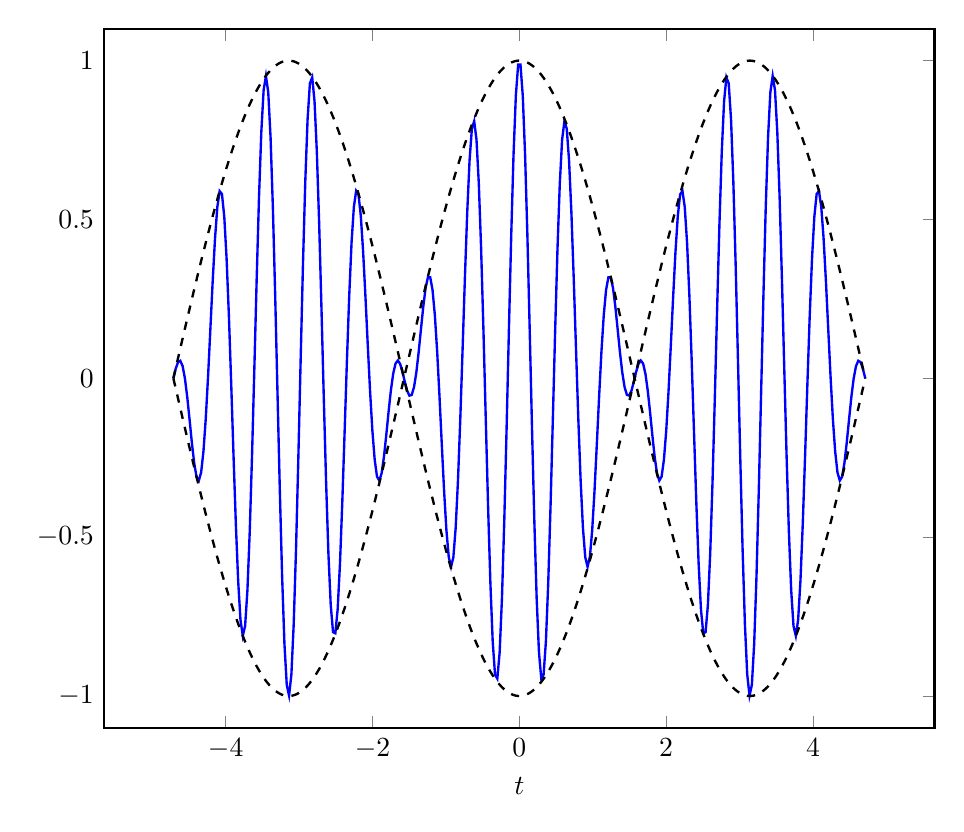
\begin{tikzpicture}
                        \begin{axis}[%
                            width=\textwidth,
                            xtick distance=1,
                            ymin=-1.1,
                            ymax=1.1,
                            xtick distance=2,
                            ytick distance=0.5,
                            line width=0.3mm,
                            ytick pos=right,
                            yticklabel pos=left,
                            xlabel=$t$
                        ]
                            \addplot[%
                                samples=300,
                                domain=-4.712389:4.712389,
                                draw=blue
                            ]
                                {cos(deg(x))*cos(deg(10*x))};
                            \addplot[%
                                samples=300,
                                domain=-4.712389:4.712389,
                                dashed
                            ]
                                {cos(deg(x))};
                            \addplot[%
                                samples=300,
                                domain=-4.712389:4.712389,
                                dashed
                            ]
                                {-cos(deg(x))};
                        \end{axis}
                    \end{tikzpicture}
                    \subcaption{Real Part of $a(t)$.}
                \end{subfigure}
                \hfill
                \begin{subfigure}[b]{0.49\textwidth}
                    \captionsetup{type=figure}
                    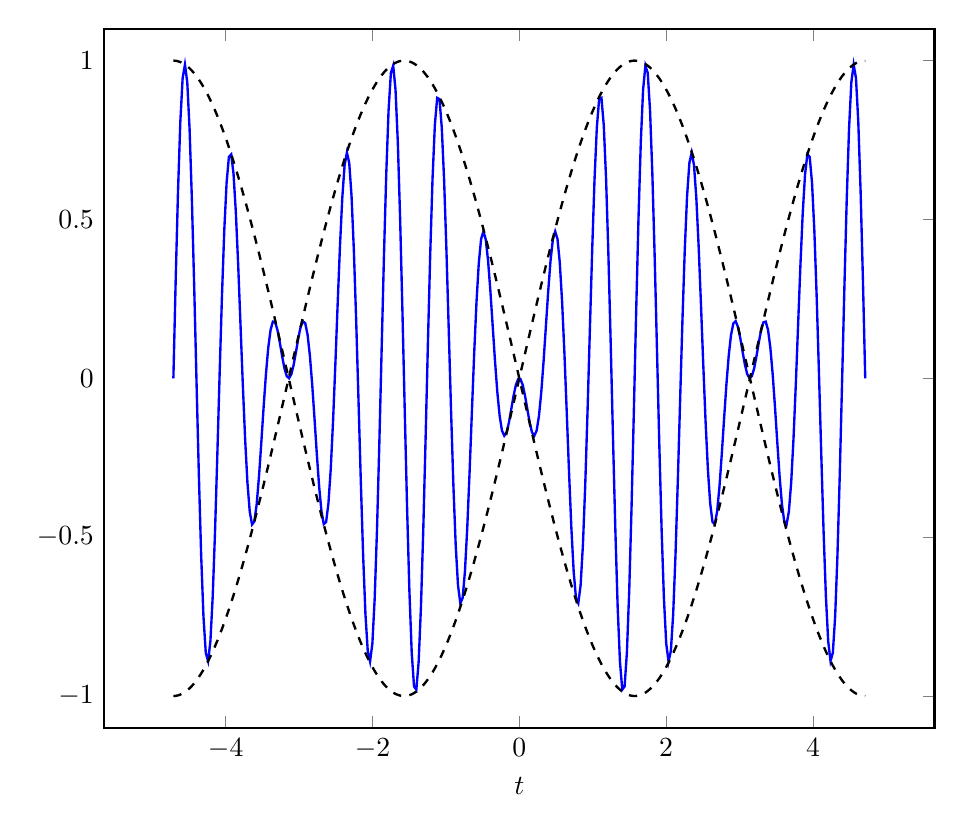
\begin{tikzpicture}
                        \begin{axis}[%
                            width=\textwidth,
                            xtick distance=1,
                            ymin=-1.1,
                            ymax=1.1,
                            xtick distance=2,
                            ytick distance=0.5,
                            line width=0.3mm,
                            ytick pos=right,
                            yticklabel pos=left,
                            xlabel=$t$
                        ]
                            \addplot[%
                                samples=300,
                                domain=-4.712389:4.712389,
                                draw=blue
                            ]
                                {-sin(deg(x))*sin(deg(10*x))};
                            \addplot[%
                                samples=300,
                                domain=-4.712389:4.712389,
                                dashed
                            ]
                                {sin(deg(x))};
                            \addplot[%
                                samples=300,
                                domain=-4.712389:4.712389,
                                dashed
                            ]
                                {-sin(deg(x))};
                        \end{axis}
                    \end{tikzpicture}
                    \subcaption{Real Part of $b(t)$.}
                \end{subfigure}
                \caption{Real Parts of the Solution to the
                         Initial Value Problem defined in
                         Eqn.~\ref{diffeq:coupled_osc_eq_1} and
                         Eqn.~\ref{diffeq:coupled_osc_eq_2}.
                         Dashed Lines
                         Represent \textit{envelopes}.}
                \label{fig:DIFFEQ:Example_of_Linear_DIFFEQ_System}
            \end{figure}